\documentclass{article}

\usepackage[a3paper,landscape,margin=5pt]{geometry}

\usepackage[utf8]{inputenc}
%\usepackage[T1]{fontenc}

%%% FONT PACKAGES
%\usepackage[scaled=0.85]{beramono} % inconsolata or beramono ???
%\usepackage{fouriernc} % serif: new century schoolbook
\usepackage{avant}     % sans serif: Avant Garde
\usepackage{microtype} % Slightly tweak font spacing for aesthetics
%\usepackage{changepage}   % for the adjustwidth environment to make narrow paragraphs

\usepackage{sectsty} %change font on headings
\allsectionsfont{\sffamily}


\usepackage{tikz}
\usetikzlibrary{calc}

\begin{document}
\thispagestyle{empty}
\renewcommand{\familydefault}{\sfdefault}


\begin{tikzpicture}[overlay,remember picture]
    \fill[red!30] (current page.south west) rectangle (current page.north east);
    \node[text width=250mm, align=right] (intro) at ($(current page.north east)+(-14.5,-4.5)$) {
       \fontsize{28}{46}\sffamily\selectfont\textbf{Introduktion~till} 
       };  
       
    \node[text width=250mm, align=right] (prog) at ($(current page.north east)+(-14.5,-6.5)$) {
       \fontsize{52}{46}\sffamily\selectfont\textbf{programmering} 
       };        

    \node[text width=250mm, align=right] (prog) at ($(current page.north east)+(-14.5,-26.2)$) {
       \fontsize{28}{46}\sffamily\selectfont{med~~Scala~~och~~Java} 
       };        
    
    \node[text width=250mm, align=right] (prog) at ($(current page.north east)+(-14.5,-27.2)$) {
       \fontsize{18}{46}\sffamily\selectfont\texttt{http://cs.lth.se/pgk} 
       };    
   

    \node[above right] (picture) at ($(current page.south east)+(-16,5.5)$) {
\includegraphics[scale=0.75]{gurka.jpg}};
    
        
    \node[anchor=north,rotate=-90, align=left] (back) at ($(current page.north)+(0.0,-13.5)$) {
    \fontsize{14}{20}\sffamily\selectfont\textbf{Introduktion till programmering med Scala och Java} \hspace{2cm}\texttt{\small https://github.com/lunduniversity/introprog}};

\node[above right] (collection-traits) at ($(current page.west)+(4.8,7.5)$) {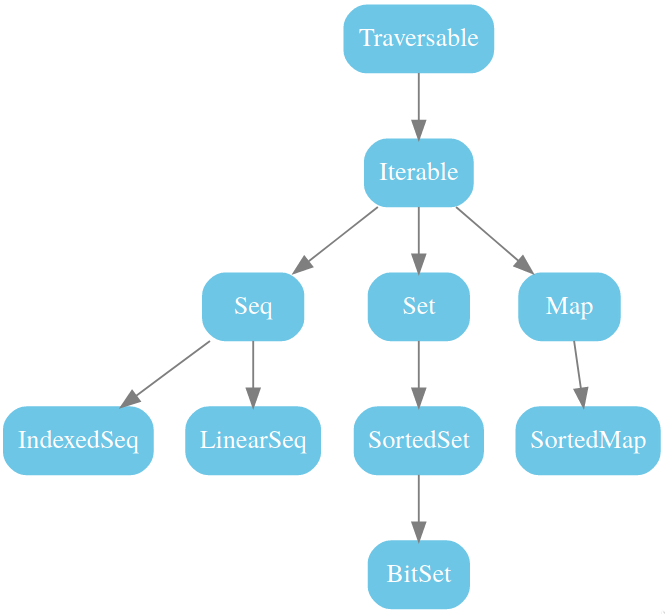
\includegraphics[scale=0.35]{../../img/collection/collection-traits}};

\node[above right] (collection-legend) at ($(current page.west)+(14,7.5)$) {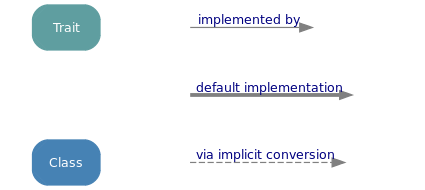
\includegraphics[scale=0.20]{../../img/collection/collection-legend}};

\node[above right] (collection-immutable) at ($(current page.west)+(4,-1.5)$) {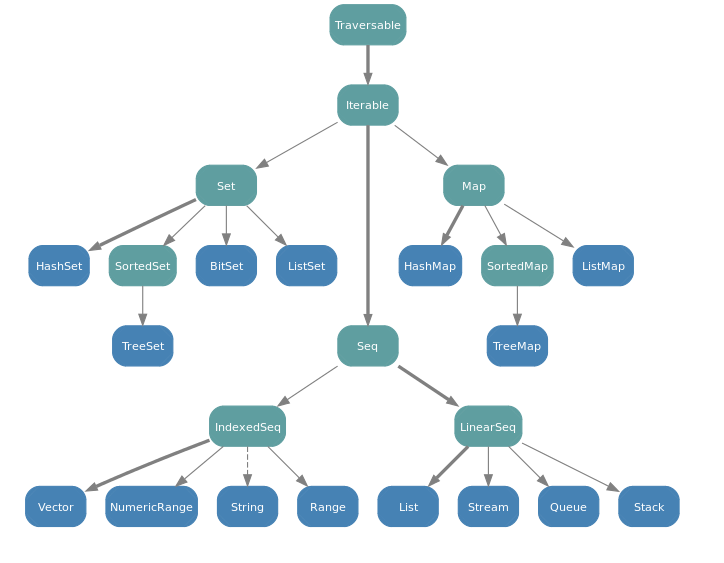
\includegraphics[scale=0.35]{../../img/collection/collection-immutable}};

\node[above right] (collection-mutable) at ($(current page.west)+(2,-13.5)$) {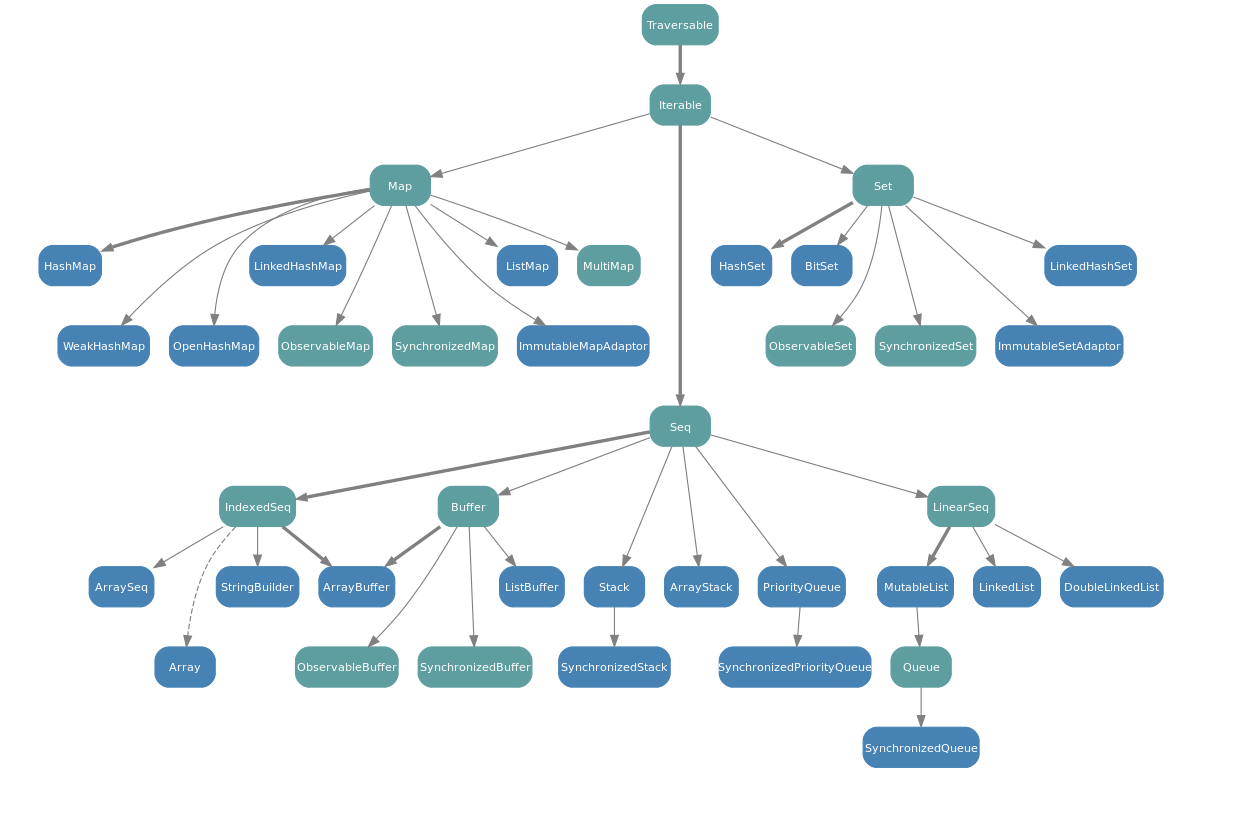
\includegraphics[scale=0.35]{../../img/collection/collection-mutable}};

\node[above right] (logo) at ($(current page.west)+(19.8,-18.5)$) {
\includegraphics[scale=0.35]{logoLUeng}};

% ../../img/collection/collection-immutable
\end{tikzpicture}
\end{document}